\documentclass[mathserif]{beamer}

\usepackage{beamerthemeshadow}
\usepackage{graphicx}
\usepackage{graphics}
\usepackage{pgf}
\usepackage{tikz}
\usetikzlibrary{arrows,automata,petri,positioning}
\usepackage[latin1]{inputenc}

\title{STAGE Prototype}
\subtitle{An event-based simulation environment}
\author{Aaron M. Rosenfeld \\ Dustin S. Ingram}
\date{\today}

\begin{document}

\frame{\titlepage}

\frame
{
    \frametitle{Personal Introduction}
    Dustin Ingram \& Aaron Rosenfeld
    \begin{itemize}
	\item Senior undergraduate Computer Science students at Drexel University, Philadelphia, PA.
	\item 2+ years at A.J. Drexel Applied Communications and Information Netrking (ACIN) Institute in the Secure Wireless Agent Testbed (SWAT) Laboratory
	\item 6 months at U.S. Naval Research Laboratory (NRL) in the Protocal Engineering Advanced Networking (PROTEAN) Research Group in Washington, DC.
	\item Previous work focusing on network protocol design and distributed network simulation \& emulation
    \end{itemize}
}

\frame
{
    \frametitle{Overview of STAGE}
    \begin{itemize}
	\item Event-based simulation environment
	\item Used to compare combinations of software agents, network configurations, and sensor data in real-world environments
	\item Physically Distributed Simulation
	\item Visualization
	\item ``Programming'' Interface:
	\begin{itemize}
	    \item Agent Software
	    \item Network Topologies
	    \item Sensor Functions
	    \item World Objects
	\end{itemize}
	\item Real networks \& Communication
	\item Bridges network emulators and agent simulators
    \end{itemize}
}

\frame
{
    \frametitle{Overview of STAGE}
    \begin{center}
        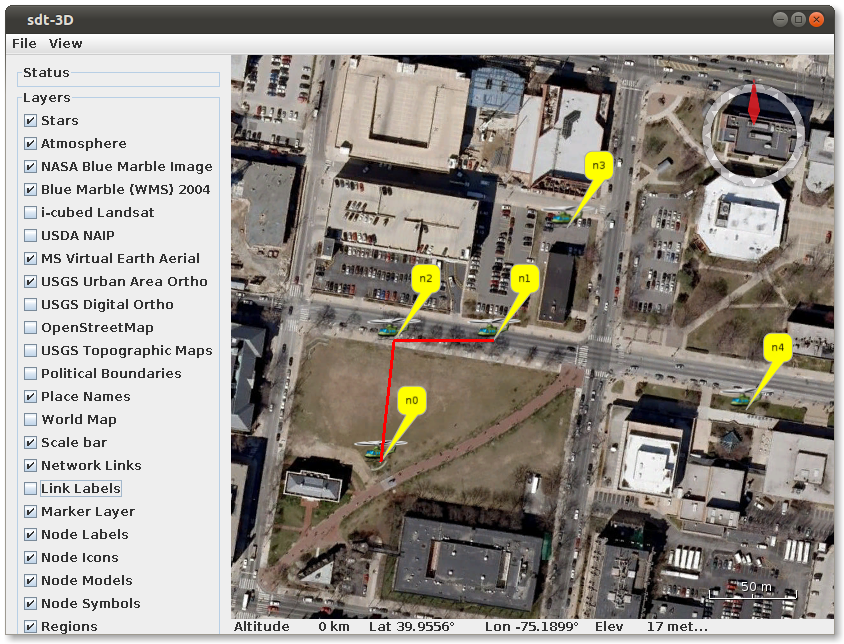
\includegraphics[scale=.3]{ss2.png}
    \end{center}
}

\frame
{
    \frametitle{Motivation}
    \textbf{Current Network Simulators}
    \begin{itemize}
	\item Existing simulation engines not designed for testing agents but for testing the network \& protocols (NS2/3)
	\item Pre-scripted scenarios (CORE) or poor event support (EMANE)
	\item Lack of templated agents
	\item Inability to batch process many executions of scenarios with varying settings
	\item Data collection non-existent or not supported
    \end{itemize}
    \textbf{Current Agent Frameworks}
    \begin{itemize}
	\item Communications modeled only at the application layer (send/recv)
	\item Lack of rich lower-level protocols
	\item Alternative approaches (Player project) require physical hardware for networking
    \end{itemize}
}

\frame
{
    \frametitle{Motivational Background - CORE}
    \begin{itemize}
	\item CORE is a network emulator which allows software to be run inside virtual machines with full network stacks
	\item Uses Linux network namespaes (netns), a lightweight container-based virtualization similar to FreeBSD ``jail''
	\item Basic implementation of PHY and MAC layer protocols including 802.11 and Ethernet
	\item Extremely easy to create scenarios; drag and drop interface
	\item Currently being developed by Boeing, based on the open source Integrated Multiprotocol Emulator/Simulator (IMUNES) project developed by the University of Zagreb
    \end{itemize}
}

\frame
{
    \frametitle{Motivational Background - CORE}
    \begin{center}
        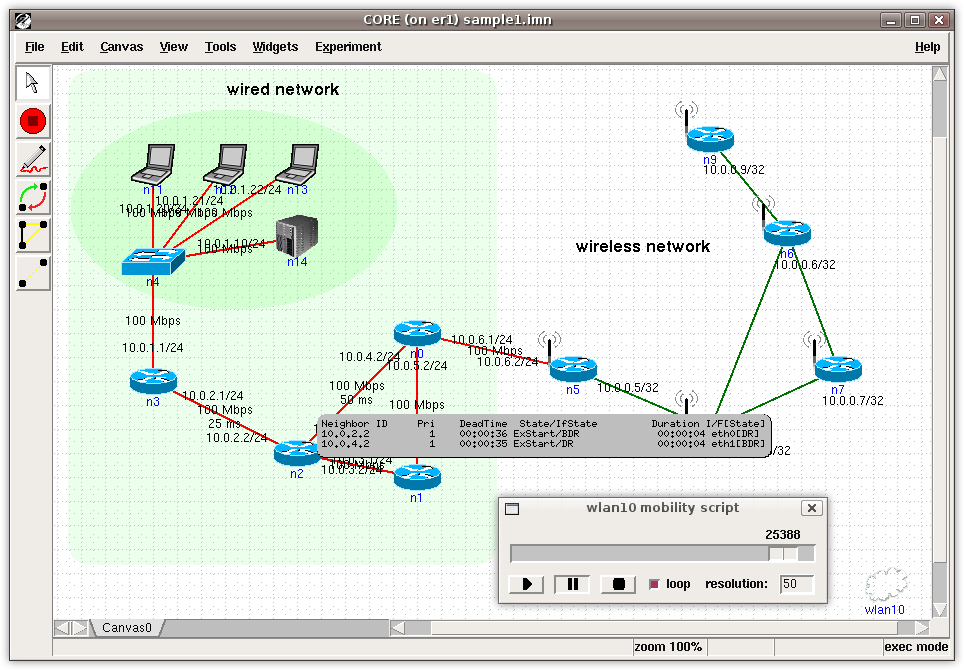
\includegraphics[scale=.3]{core-screenshot.png}
    \end{center}
}

\frame
{
    \frametitle{Motivational Background - EMANE}
    \begin{itemize}
	\item EMANE is an Extendable Mobile Ad-hoc Network Emulator
	\item Allows heterogeneous network emulation using a plugable MAC and PHY layer architecture
	\item Pre-scripted scenarios publich timed events to a common event channel
	\item 1-to-1 virtual-to-physical node mapping (without additional virtualization)
	\item No GUI or integrated visualization component
	\item EMANE is an Open Source project developed by CenGen, Inc., Columbia, Maryland and released under the BSD license
    \end{itemize}
}

\frame
{
    \frametitle{Motivational Background - NS3}
    \begin{itemize}
	\item Well known network simulator with proven accurate network stack characteristics
	\item Command line based
	\item Allows developers to write applications and define scenarios in C/C++
	\item Simulated -- results in slower-than-realtime experiments
	\item Applications must be written from scratch; no notion of agents or modularity
    \end{itemize}
}

\frame
{
    \frametitle{Goals}
    \textbf{Bridge gap between agent and network simulation}
    \begin{itemize}
        \item Allow for human-in-the-loop interaction
	\item Enable mixing-and-matching of template agents (e.g. camera, radar, wave sensor)
        \item Make writing custom agents extremely simple
        \item Enable scenarios and network topologies to be easily defined
        \item Entirely event-driven
        \item Agents can be intelligent, pre-scripted, or live-feeds
        \item Visualization flexibility
        \item Distributed
        \item Modular communication interface to allow future integration of high-quality network models (NS3)
    \end{itemize}
}

\frame
{
    \frametitle{Proposed Architecture}
    \begin{center}
        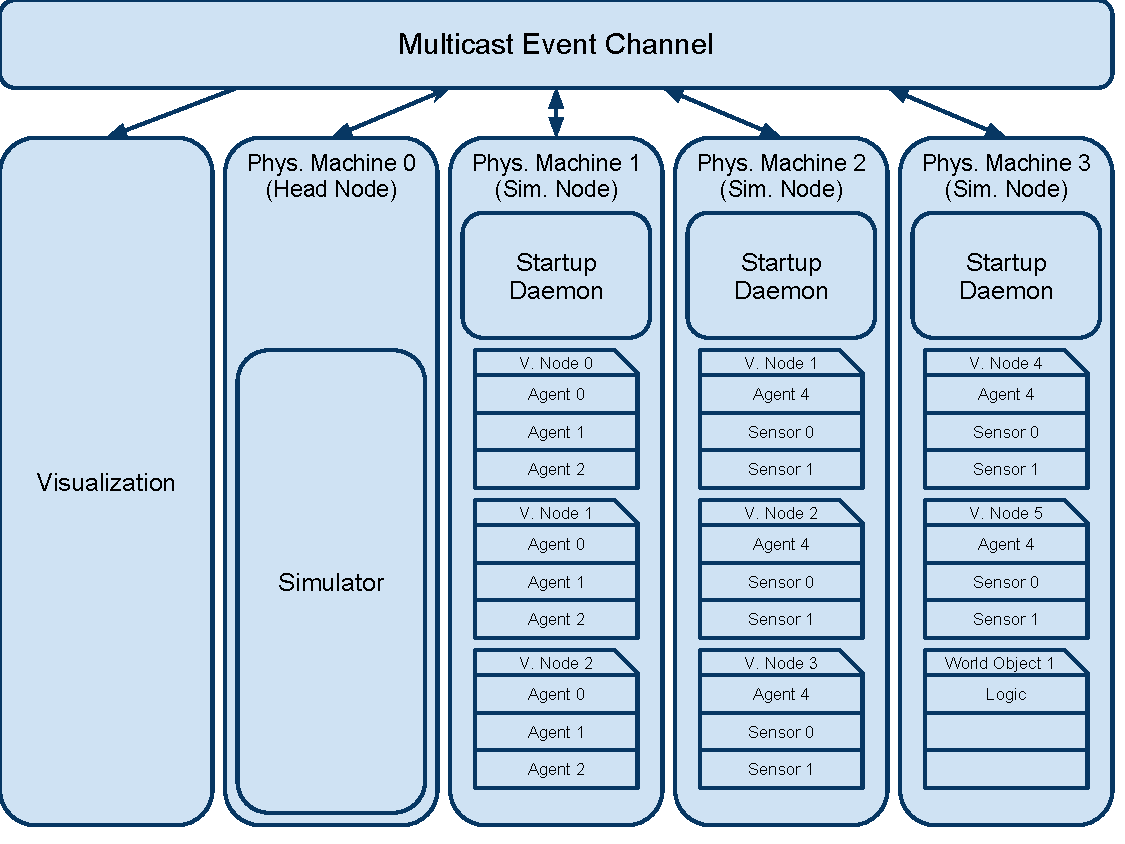
\includegraphics[scale=.5]{CTUSeminar.pdf}
    \end{center}
}

\begin{frame}[fragile]
    \frametitle{Example Scenario Definition}
    Scenario creating five nodes, each with an ``Example'' agent:
    {\small
    \begin{verbatim}
class ScenarioExample(Scenario) :
    def __init__(self) :
        Scenario.__init__(self)
        for node_id in range(0, 5) :
            node = Node(name='n%s' % node_id, \
              position=(0,0,0), agents = [ExampleAgent()])
            
            self._nodes.append(node)
    \end{verbatim}}
\end{frame}

\begin{frame}[fragile]
    \frametitle{Example Network Definition}
    Network definition adding a wireless interface to each of nodes in a scenario:
    {\small
    \begin{verbatim}
class NetworkExample(Network) :
    def __init__(self, scen_inst) :
        Network.__init__(self, scen_inst)
        for node in self._scen_inst.get_nodes() :
            node.get('interfaces')['eth0'] = \
              Interface(type='wireless', power=50, \
              ssid='wlan0')
    \end{verbatim}}
\end{frame}


\begin{frame}[fragile]
    \frametitle{Example Custom Agent Definition}
    Example agent which randomly sets waypoints within a 100m square of its containing node, waits for the movement to complete, and repeats:
    {\small
    \begin{verbatim}
class AgentExample(Agent) :
    def __init__(self, parent_node) :
        Agent.__init__(self, parent_node)
        # Any pre-configuration here
        # ...

    def run(self) :
        # Called when simulation begins
        while True :
            self._api.request_translate(random.randint(-50,50), \ 
              random.randint(-50,50))
            self._api.get_event_channel().block_until(\
              self.get_parent(), 'move_complete')
    \end{verbatim}}
\end{frame}

\begin{frame}[fragile]
    \frametitle{Template Agent \& Subscription}
    Example template agent for following a specific node:
    {\small
    \begin{verbatim}
class FollowAgent(Agent) :
    def __init__(self, parent_node, follow_id, follow_close) :
        Agent.__init__(self, parent_node)
        self._follow_id = follow_id
        self._follow_close = follow_close

    def _on_move(self, event) :
        if event.get('node_id') == self._follow_id :
            dest = self._api.get_position(self._follow_id)
            self._api.request_translate(dest)

    def run(self) :
        if self._follow_close :
            event_name = 'move_tic'
        else :
            event_name = 'move_complete'
        self._api.get_event_channel().subscribe(event_name, \
          self._on_move)
    \end{verbatim}}
\end{frame}

\frame
{
    \frametitle{Distribution}
    \textbf{Virtual Nodes}
    \begin{itemize}
	\item Very simple to distribute as all events are broadcast over a common event channel
	\item Future prototype will include method of starting agents on multiple physical machines
	\item Synchronization of simulation-time across physical machines may prove difficult, especially with integration of NS3; possible issues with human-in-the-loop
    \end{itemize}
    \textbf{Simulation Engine}
    \begin{itemize}
	\item Simulation engine may become a bottleneck as all ``filter \& forward'' (e.g. messaging) type events must flow through it
	\item Distribution of simulation engine is a future goal 
    \end{itemize}
}

\frame
{
    \frametitle{Batch Experimentation}
    \begin{itemize}
        \item Collect data from each experiment
        \item Provide tabulated results of high level metrics (e.g. data sent, packets lost)
        \item Incorporate into API to allow agents to output low-level, specific information (e.g. algorithm
        performance)
    \end{itemize}
    \textbf{Method 1}
    \begin{itemize}
        \item Provided various input parameters (e.g. number of nodes, agent configuration) and argument vector, run
        experiments
        \begin{itemize}
            \item $P := [ NodeCount, AgentArg1, AgentArg2 ]$
            \item $A := [ \{5, 10, 20\}, \{.1, .2, .5\}, \{1, 2, 3\} ]$
        \end{itemize}
    \end{itemize}
    \textbf{Method 2}
    \begin{itemize}
        \item Provide desired distributions/counts for output metrics
        \begin{itemize}
            \item ``Run each experiment until output of agent 1 fits a nearly normal distribution''
        \end{itemize}
    \end{itemize}
}

\frame
{
    \frametitle{Current Status}
    \begin{itemize}
	\item Initial requirements established
	\item Very early beta
	\item Prototype created demonstrating:
        \begin{itemize}
	    \item ``Custom'' agent definition
	    \item Network definition
	    \item Scenario definition
	    \item Visualization
	    \item Event channel
        \end{itemize}
    	\item Distribution of agents currently feasible once startup daemon is complete
    \end{itemize}
}

\frame
{
    \frametitle{Possible Collaboration Points}
    \begin{itemize}
	\item Consolidation of agent frameworks
	\item Currently omitting physics; limited to real-world topologies
	\item Visualization engine
	\item Abstraction of Agent/Mobility definition language
    \end{itemize}
}

\frame
{
    \frametitle{Contact \& Links}
    \begin{center}
	Dustin S. Ingram\\
	\texttt{dsi23@drexel.edu} \\

	Aaron M. Rosenfeld \\
	\texttt{ar374@drexel.edu} \\
    \end{center}

    \textbf{STAGE:} http://code.googe.com/p/stage \\
    \textbf{CORE:} http://cs.itd.nrl.navy.mil/work/core \\
    \textbf{EMANE:} http://cs.itd.nrl.navy.mil/work/emane \\
    \textbf{NS3:} http://www.nsnam.org  \\
}

\end{document}
